\documentclass{article}
\usepackage{fullpage}
\usepackage{graphicx}
\begin{document}

\title{Software Requirements Specification for Mashbot} 
\author{George D'Andrea \and Andrew Gall \and Josiah Kiehl \and
  Cody Ray \and Vito Salerno}
\date{\today}
\begin{titlepage}
\maketitle
\end{titlepage}

\section*{Revision History}
\begin{tabular}{|p{2in}|l|l|l|}
  \hline
  \textbf{Name} & \textbf{Date} & \textbf{Reason for Changes} & \textbf{Version} \\
  \hline \hline
  George D'Andrea, Andrew Gall, Josiah Kiehl, Cody Ray, Vito
  Salerno & 16 February 2010 & Revised from Reviews & 1.1 \\
  \hline
  George D'Andrea, Andrew Gall, Josiah Kiehl, Cody Ray, Vito
  Salerno & 24 November 2009 & Initial Version & 1.0 \\
  \hline
\end{tabular}

\clearpage
\tableofcontents
\clearpage

\section{Introduction}

\subsection{Purpose} % JK
This document is the general overview of the software requirements for
the Mashbot project. These requirements are directly related to the
functionality, performances, constraints, attributes, and interfaces
of the system.

Mashbot is a web service for managing a company's presence on social
networks. One goal of Mashbot is to unify the interfaces of a
multitude of social networks, allowing users to learn a standardized
interface and more easily cope with the flood of new social network
platforms. A second goal is to allow for a hands off approach to
social network marketing by allowing the scheduling of campaign events
to be distributed to social networks.
 
\subsection{Scope} % JK
This document contains the criteria by which the initial Mashbot
release will be judged. It is written for the developers, testers, and
end-users of Mashbot.
\subsection{Glossary} % Everyone

\begin{itemize}

\item \textbf{Campaign} A collection of content that is scheduled to be
published
\item \textbf{External Service Account} An account on a social
  networking platform outside of Mashbot

\end{itemize}

\subsection{Overview} % CR

Marketing, customer service, business overhead and development efforts
compete for resources in many startups and small
businesses. Furthermore, early stage startups often have small or
non-existent marketing budgets, especially in resource-hungry
product-based startups. Although the plethora of widely available and
affordable communications technology (e.g., social media, VoIP,
streaming video, etc.) theoretically reduces both capital and
operating expenditures related to marketing, the quantity of such
technologies and services effectively creates an "opportunity
overload" which makes the process of maintaining a focused and
effective marketing campaign more difficult. Furthermore, with the
number of services, technologies, and "specialists" arriving each day,
it is nearly impossible to keep up with all the trends, much less
fully take advantage of each one, or even monitor them all
adequately. The widespread adoption of communications technology is a
double-edged sword; there are many more avenues for marketing and
customer service, but it is much more difficult to effectively apply
reputation management strategies or adequate customer service through
all channels. This project proposes to build a tool to increase the
effectiveness and efficiency of marketing campaigns and customer
service for small to medium businesses.

\section{Overall Description}
     \subsection{Product Perspective} % CR

The initial focus will be on scheduled marketing campaigns utilizing
social media. However, this may expand to include customer service
functionality, management of more traditional campaigns such as
direct mail, trade shows and other events, or user-created campaign
classes.
 
The first objective is to develop and release a small open source
platform to provide a service agnostic facade API bundling common
operations in widely used services (e.g., Facebook, Flickr, Twitter,
Wordpress, or YouTube). This platform will provide a plugin-based
architecture for abstracting myriad services behind a single facade,
based upon content types provided in common data models. This
sub-project will not only be useful to the open source community but
will also devalue much of the competition whose prime added value
comes from providing such a service. Furthermore, it opens the
opportunity for the public to help maintain existing service plugins
as well as contribute plugins for new services. Finally, it leads to
the inclusion of both a dual licensing revenue model and a niche
software development service-based revenue model for custom extensions
and applications built upon this core, which is proven to be more
sustainable over time.
 
The first application of this core platform will be the campaign
manager referenced above.  While the exact feature set is to be
determined during the design process, expected features include a
portal to existing services where messages can be "pushed", or
broadcast, through existing service channels. This portal will also
allow for the collection of responses from customers, fans, critics,
and other audiences from these same channels. Users will be able to
view social networking messages directed at them, as well as perform
data mining tasks on the social networks to provide more intelligent
heuristics regarding brands' strength amongst particular markets. They
will also be allowed to schedule campaign events at certain times. For
example, users will be able to prepare a press release far in advance
of its distribution, or queue a number of updates to be spread out
over a certain time period.

\subsubsection{System Interfaces} % VS
Mashbot combines several components to provide required functionality.
\begin{itemize}
\item \textbf{Authentication} Mashbot will allow the use of external
  authentication modules for user login. Mashbot will also provide an
  internal authentication mechanism in case an external module is
  unavailable.
\item \textbf{Campaign Manager Web Client} Mashbot has an interface
  for a web client which processes user commands to interact with
  campaigns.
\item \textbf{Publishing and Aggregation Platform} Mashbot has an
  interface for publishing content to social networks, as well as for
  aggregating social network data.
\item \textbf{Database} Mashbot has an interface to a database which
  allows for the storage and retrieval of data related to accounts and
  campaigns.
\end{itemize}
\subsubsection{User Interface} % JK
The user interface consists of a web front end with tabs to separate
the various workflow areas. To create content, the user is provided
with a calendar scheduling tool and a content editor.  Additionally,
there is a monitoring dashboard which gives the user a view on
responses to the content in any given campaign.  Finally, there is an
explore view that gives the user a portal with which they can keep
tabs on topics of interest in social media.
\subsubsection{Hardware Interfaces} % VS
The Mashbot web client runs on any computer hardware meeting the
following criteria:
\begin{itemize}
\item Capable of connecting to the Internet
\item Capable of running a modern HTTP 1.1 web browser
\item Includes a keyboard and a pointing device
\item Includes writable volatile storage
\end{itemize}
The Mashbot server runs on any computer hardware meeting
the following criteria:
\begin{itemize}
\item Capable of connecting to the Internet as a server.
\item Capable of interfacing with modern database software.
\item Capable of running a modern suite of networking software.
\end{itemize}

\subsubsection{Software Interfaces} % VS
The Mashbot software integrates some external software to provide
functionality.
\begin{itemize}
\item \textbf{Authentication} Mashbot authenticates users against it's
  internal user database.
\item \textbf{Campaign Manager Web Client} Mashbot interfaces with the
  user’s web browser and expects that it is capable of HTTP 1.1 and
  HTML 4.0.
\item \textbf{Database} Mashbot software interfaces with an existing
  database software.
\item \textbf{Publishing and Aggregation Platform}
\item \textbf{Server} The Mashbot server runs on an operating system
  that supports serving dynamic web pages using encryption and is
  capable of communicating with the Internet.
\end{itemize}
\subsubsection{Communications Interfaces} % VS
Communication between the web client and the server software is
facilitated by common network protocols. This allows compatibility
with the majority of our user's machines.  Data will be encrypted
using TLS and HTTP/1.1. The use of these protocols requires the
ability for the systems to communicate using TCP/IP network stacks.
The Mashbot system sends emails using SMTP.

\subsubsection{Memory Constraints} % VS
The Mashbot server requires no greater than 1 gigabyte of RAM
memory. The web client requires no more than the minimum memory a
modern desktop computer commonly has, approximately 256 megabytes of
RAM.

\subsection{Product Functions} % AG
Mashbot should be able to:
\begin{enumerate}
\item Schedule content for various services to be published
  concurrently
\item View and Compare historical metrics of campaigns
\item View/Create replies to content
\item Maintain users and approvers of content
\item Set up keyword alerts for ``watched'' services
\end{enumerate}
\subsection{User Characteristics} % AG
The target user is a small to medium business employee who understands
the basic capabilities of social media.

\subsection{Requirements Apportioning} % VS
\begin{tabular}{|c|p{4in}|}
  \hline \textbf{Priority} & \textbf{Description} \\ \hline \hline 1 &
  Mashbot can not be released unless it satisfies these
  requirements. \\ \hline 2 & Mashbot may be initially released
  without satisfying these requirements. Having these requirements
  unfulfilled must not create dangers to the system. They should be
  implemented in the next minor release. \\ \hline 3 & These
  requirements are not expected to be fulfilled by the initial release
  of Mashbot, but should be implemented in the next major
  release. \\ \hline 4 & These requirements are outside the current
  scope of the project, but are included to exhibit how our software
  will improve in the future. \\ \hline
\end{tabular}

\section{Specific Requirements}
\subsection{External Interface Requirements} % DO THIS
\subsubsection{Email System}
\begin{description}
\item[0100] \textbf{Purpose} The external email system is to provide a
  messaging service from Mashbot to the Mashbot
  users. \textbf{Priority 2}
\item[0110] \textbf{Input} The input is generated automatically by the
  Mashbot system using settings configurable by the System
  Administrator. \textbf{Priority 2}
\item[0120] \textbf{Output} The output is in the form of an e-mail to an
  e-mail account, but it does not return any sort of message to
  Mashbot. \textbf{Priority 2}
\item[0130] \textbf{Data Format} The format uses SMTP protocol. The actual
  messages are provided by Mashbot. \textbf{Priority 2}
\end{description}

\subsection{Functional Requirements}
\subsubsection{User Accounts} % AG
\begin{description}
\item[0140] \textbf{User Account Types and Permissions} The system
  categorizes users on the basis of roles and privileges. Within these
  roles, the system also categorizes users based on the roles that
  they have within individual products. These are referred to as user
  account roles.

  \begin{description}
  \item Mashbot Campaigns supports the following account roles:
    
    \begin{description}
      \item[0150] Contributor \textbf{Priority 3}
      \item[0160] Approver \textbf{Priority 3}
      \item[0170] Publisher \textbf{Priority 3}
    \end{description}

  \item[0180] A user may possess more than one role. \textbf{Priority 3}
  \item[0190] Roles reflect actions that can be performed by a
    user. \textbf{Priority 3}
  \item[0200] Roles can be assigned to a user account for individual
    products. \textbf{Priority 3}
  \item[0210] \textbf{Contributors} may create new content, import
    existing content into the system, edit content, and delete
    it. They may also submit these actions for approval. \textbf{Priority 3}
  \item[0220] \textbf{Approvers} can approve actions performed by
    contributors \textbf{Priority 3}
  \item[0230] \textbf{Publishers} may schedule or immediately initiate
    actions put forth by contributors and those approved by approvers.
    \textbf{Priority 4}
  \end{description}
  
  \item[0240] \textbf{User Account Creation} - New user accounts can be
  created. \textbf{Priority 1}

  \begin{description}
  \item[0250] The system may contain any number of user
    accounts. \textbf{Priority 1}
  \item[0260] Certain pieces of information are required to create new
    accounts. \textbf{Priority 1}
  \item The following information is required for any new user
    account:

    \begin{description}
    \item[0270] Username \textbf{Priority 1}
    \item[0280] Password \textbf{Priority 1}
    \item[0290] Name \textbf{Priority 1}
    \item[0300] Email Address \textbf{Priority 1}
    \item[0310] Group Membership \textbf{Priority 1}
    \item[0320] User Account Type \textbf{Priority 1}
    \end{description}

  \end{description}

  \item[0330]\textbf{User Account Modification} The system allows users to
    modify their accounts once created. \textbf{Priority 1} 

    \begin{description}

  \item[0340]The system requires that a user have logged in before
    modifications can be made. \textbf{Priority 1}
  \item The following user account information is modifiable by all
    user types:

    \begin{description}
    \item[0350]Password \textbf{Priority 1}
    \item[0360]Email Address \textbf{Priority 1}
    \item[0370]Name \textbf{Priority 1}
    \end{description}
    \end{description}

    
  \item[0380] \textbf{User Account Deactivation} The system allows user
    accounts to be deactivated. \textbf{Priority 3}

    \begin{description}

    \item[0390] The system denies user who have been deactivated from
      accessing the system. \textbf{Priority 3}
    \item[0400] If an account has any history associated with it, it can only
      be deactivated and not deleted. \textbf{Priority 3}
    \item[0410] If an account has no history associated with it, it can be
      deleted from the system. \textbf{Priority 3}
    \item[0420] A disable account can be undisabled \textbf{Priority 3}
    \item[0430] It is possible to disable all accounts except for the System
      Administrator account. \textbf{Priority 4}
    \end{description}

  
\item[0440] \textbf{Username and Passwords}

  \begin{description}

  \item[0450] The system gives users the ability to reset their password. \textbf{Priority 2}
  \item[0460] Individual passwords can be reset. \textbf{Priority 2}
  \item[0470] The system only allows users to change their own
  passwords. \textbf{Priority 2}

  \end{description}

\end{description}
\subsubsection{Marketing Campaigns} % JK
\begin{description}

\item[0480] A campaign has the following components:

\begin{description}
\item[0490] Name \textbf{Priority 1}
\item[0500] Pieces of content \textbf{Priority 1}
\item[0510] Schedule \textbf{Priority 1}
\item[0520] User/Group Permissions \textbf{Priority 2}
\end{description}

\item[0530] A schedule is a mapping of times to publishing actions. It may
  contain any actions a publisher can perform, and these actions are
  performed at the associated time. \textbf{Priority 1}

\item[0540] A piece of content may take the following forms:
\begin{description}
\item[0550] Text \textbf{Priority 1}
\item[0560] Image \textbf{Priority 1}
\item[0570] Audio \textbf{Priority 3}
\item[0580] Video \textbf{Priority 3}
\end{description}
\end{description}

\subsubsection{External Service Accounts} % JK

\begin{description}
\item[0590] Mashbot will allow for the association of Mashbot accounts with
  external service accounts.

\item[0600] Mashbot will provide an interface for authenticating a user
  account to an external service account \textbf{Priority 1}
\item[0610] Mashbot will provide a standardized method of interacting with
  external service accounts \textbf{Priority 1}
\end{description}

\subsection{Security Requirements} % VS
\begin{description}
\item[0620] The system encrypts data over a direct connection between the
  web client and the server.  Priority 1
\item[0630] The system allows for the backup of the data system to local or
  remote non-volatile storage systems.  Incremental backups should not
  create outages and full backups do not interfere with user
  interaction for more than 10 minutes. Priority 1
\item[0640] The system is configurable to e-mail warnings about multiple
  failed login attempts from the same user. These warnings are sent to
  the System Administrator. Other security risks of this type are the
  responsibility of the System Administrator. Priority 3
\item[0650] The system allows only valid users to log into the system. A
  valid user is one which has not been disabled or deleted and exists
  on the system. Priority 1
\item[0660] To log onto the system, a user provides their valid username and
  password. Priority 1
\item[0670] The system uses the configured authentication module. The
  authentication method is configurable by the System
  Administrator. Priority 1
\item[0680] The system allows the System Administrator to configure a
  timeout after which a user is automatically logged out of
  Mashbot. Priority 1
\end{description}

\section{User Interface} % JK
The user interface will consist of a tabbed navigation bar that
unifies the sitewide navigation, as well as module specific navigation
as needed. Tabs:
\begin{itemize}
\item Dashboard
\item Create
\item Schedule
\item Explore
\end{itemize}
\subsection{Dashboard}
The dashboard consists of graphs and charts to give the user a quick
view on how their campaigns are performing.  Metrics include:
\begin{itemize}
\item Clickthrough rate
\item Page Views
\item Number of Comments
\end{itemize}
Service plugins can define additional specialized metrics to track, as
well, for instance ``retweets'' for Twitter.  A panel is available to
give more information on each metric as it is selected. See Fig~\ref{dashboard}
\subsubsection{Create}
This view allows users to create campaigns and fill them with content.
This view is also used when users need to edit an existing
campaign. See Fig~\ref{create}
\paragraph{Add content}
A user can add content via the add content button near the top of the
view.  This will prompt the user to select the content type, which is
populated by the services the user currently has access to via
credentials stored in the system. This will create a section in the
main part of the view that allows the user to add individual elements
of that content type, each individually scheduled.  Each row line item
will allow the user to schedule, edit, or delete that content type.
\subsubsection{Schedule}
\paragraph{Scheduling content}
Users can drag items from the left hand bucket of content to the
calendar to schedule content.  The content will receive a default
golive time of 12am on the day the content is dragged to.  If the user
desires a different time, he may click the content in the schedule and
assign the proper time. See Fig~\ref{schedule}
\paragraph{Calendar}
The calendar allows the user to manage when content goes live, and
gives a visual representation of the actions taken on content.  It is
clear when content goes live and when (if) it is deleted.  The user
can page from month to month to schedule content to any day desired.
\subsubsection{Explore}
This view allows users to get a pulse on what information social media
contains.  This includes the ability to set up monitored searches for
services that support keyword search via api.  This also will
aggregate data gathered from comments on content that has been
published as part of a given campaign
\clearpage
\begin{figure}
\centering
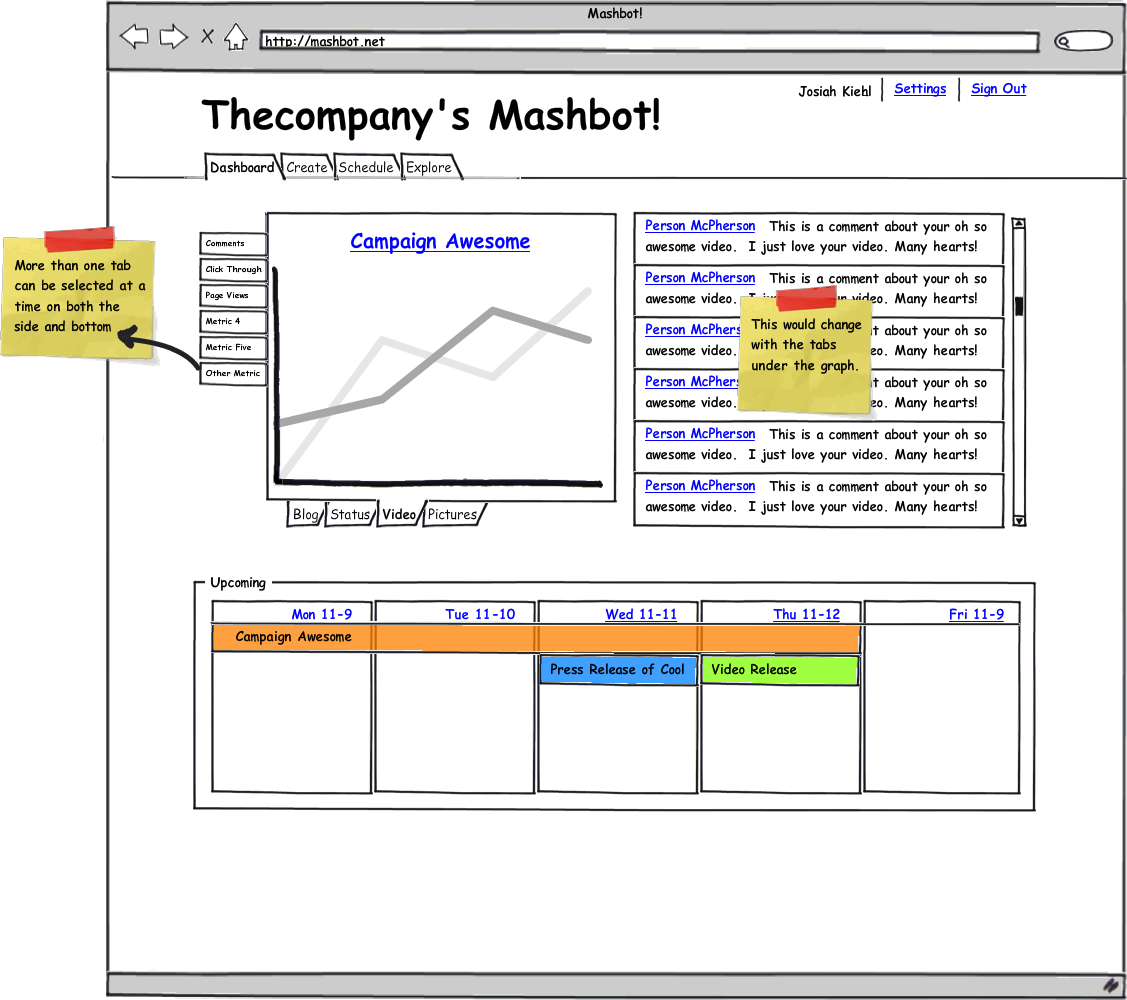
\includegraphics[scale=0.35]{../mockups/dashboard.png}
\caption{The dashboard interface}
\label{dashboard}
\end{figure}
\clearpage
\begin{figure}
\centering
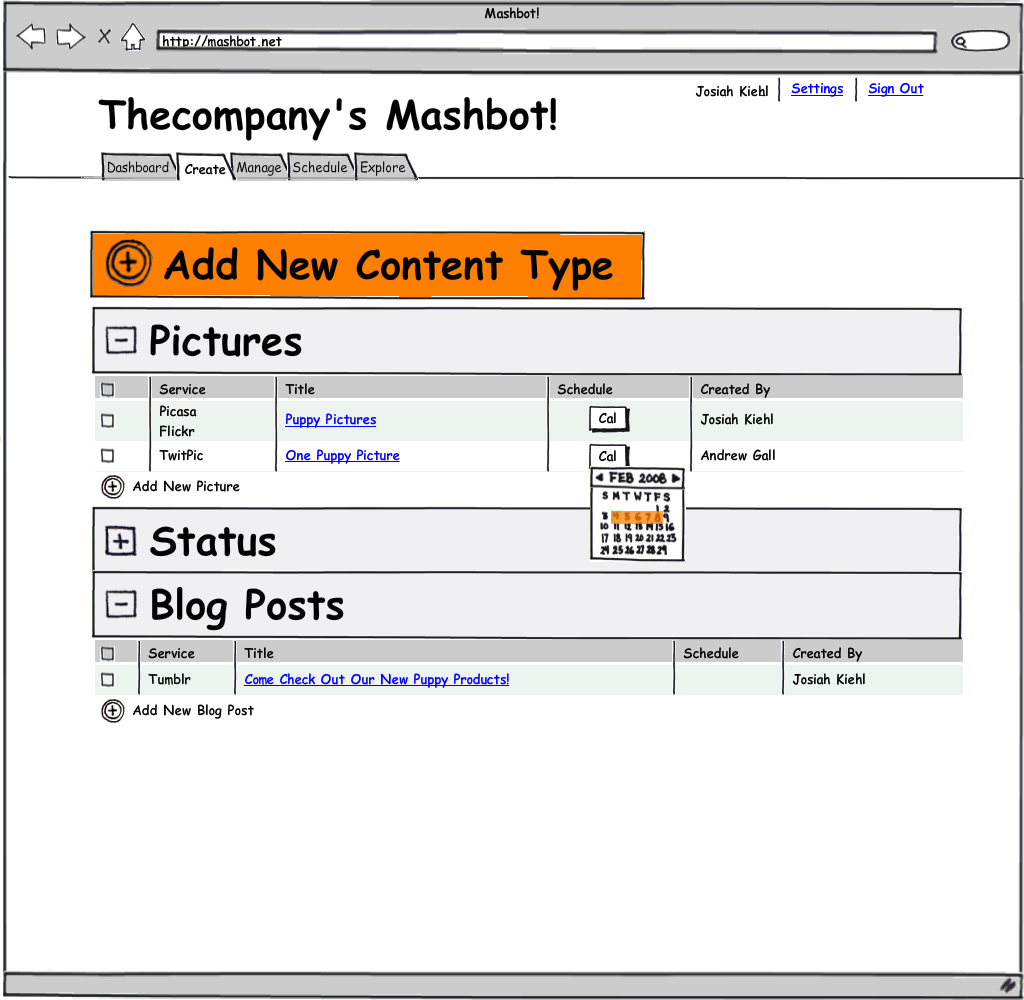
\includegraphics[scale=0.35]{../mockups/create.png}
\caption{The content creation interface}
\label{create}
\end{figure}
\clearpage
\begin{figure}
\centering
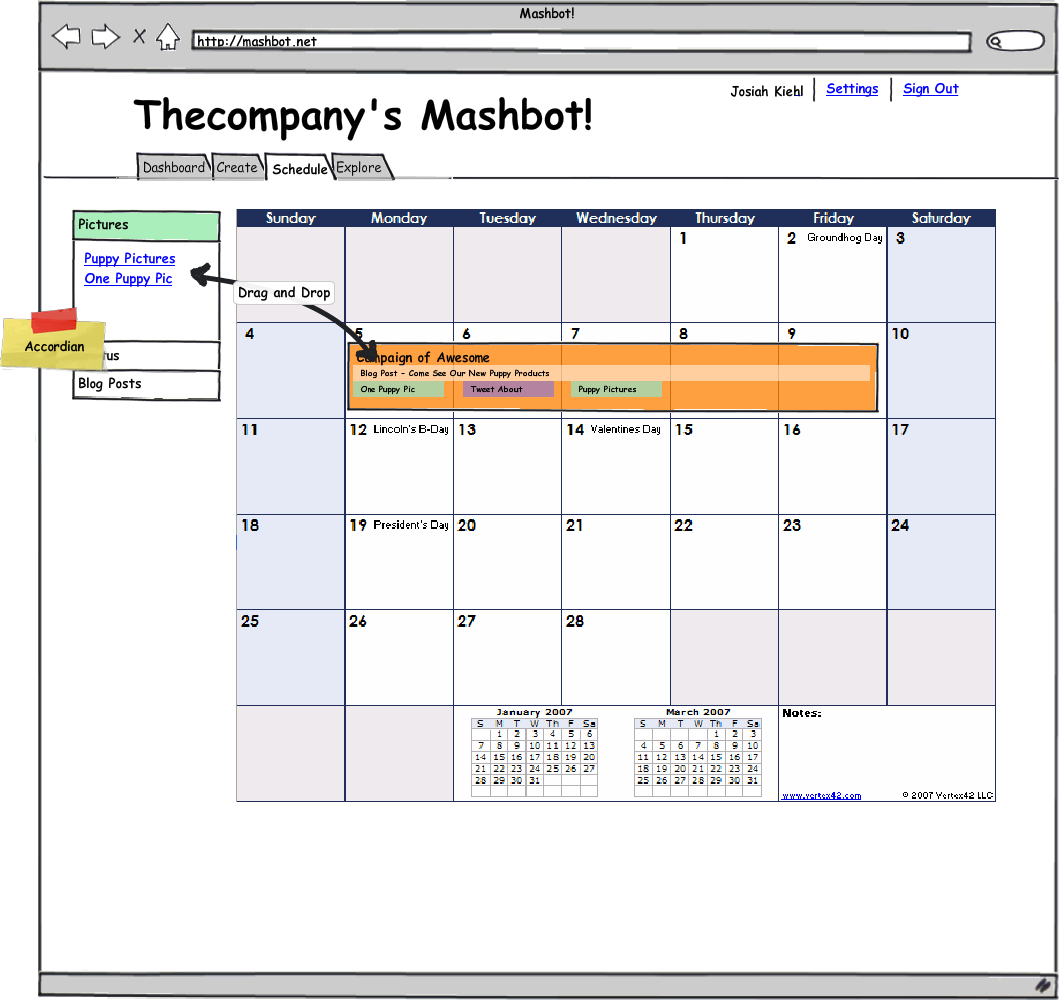
\includegraphics[scale=0.35]{../mockups/schedule.png}
\caption{The scheduling interface}
\label{schedule}
\end{figure}
\clearpage
\section{Preliminary Analysis} % JK
Mashbot is a data driven web application.  It aggregates data from
various web services.  This figure shows the flow of data through the
web application.  There is a core that handles all requests for
various data needed by the application.  Authentication information is
retrieved from the database and used to request content from services.

\begin{figure}
\centering
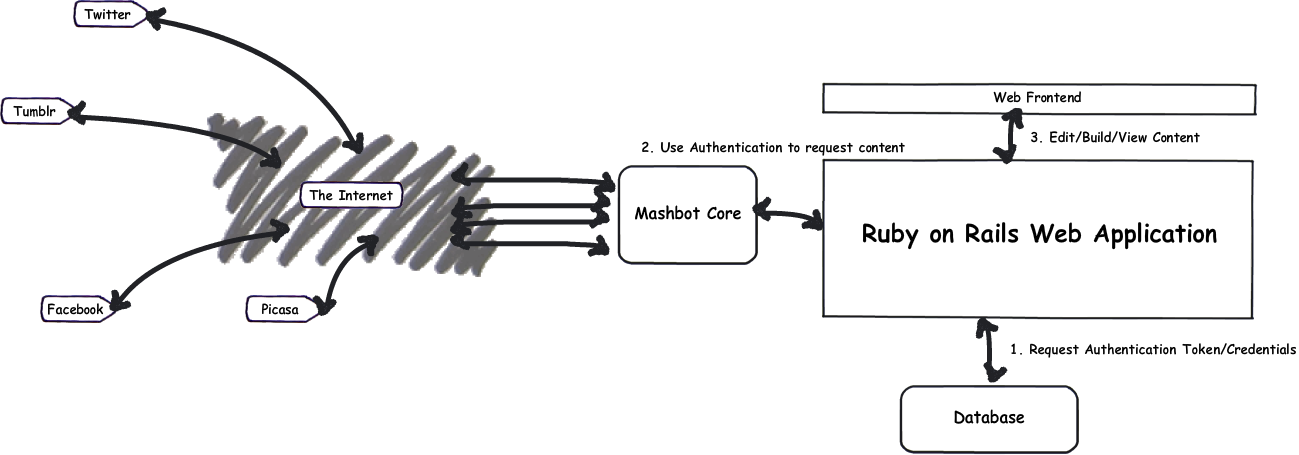
\includegraphics[scale=0.3]{../mockups/dataflow.png}
\caption{The Data Flow}
\end{figure}
\begin{figure}
\label{dataflow}
\end{figure}

\section{Use Cases} % CR
\begin{enumerate}
\item A user should be able to register a new account
\item A user should be able to log in
\item A member should be able to log out
\item A member should have a profile
\item A member should be able to modify their profile
\item A user's email should be verified when registering a new
  account.
\item An admin should be able to modify accounts
\item An admin should be able to suspend accounts
\item An admin should be able to delete accounts
\item A member should be able to monitor trending topics regarding
  their campaign
\item A member should be able to monitor facebook groups related to
  campaigns
\item A member should be able to view @replies to tweets related to
  their campaigns
\item A member should be able to see responses to blog posts related
  to the campaign.
\item An admin should be able to perform user account actions in bulk
\item An admin should be able to see all campaigns
\item An admin should be able to delete any campaign
\item An admin should be able to edit all campaigns
\item Mashbot campaigns! campaigns should allow multiple users to
  collaborate on a campaign
\item Mashbot campaigns! should support multiple users
\item A member should be able to store authentication for supported
  services
\item A member should be able to add additional services to an
  existing campaign
\item A member should be able to delete individual campaign elements
\item Members should have hierarchical permissions
\item A campaign should have workflow approval process
\item A member should be able to "unpublish" a campaign
\item A member should be able to delete a campaign
\item A member should be able to schedule events in bulk
\item A member should be able to schedule "live dates" for individual
  events.
\item A member should be able to delete existing content from
  supported services
\item A member should be able to see the content they have published
  in all supported services
\item A member should be able to push to Facebook in a campaign
\item A member should be able to post to a blog in a campaign
\item A member should be able to post to Twitter in a campaign
\item A member should be able to create a new campaign
\item A member should get notified when activity occurs in a campaign
  they're working on
\end{enumerate}

\end{document}


% LocalWords:  Mashbot
